\documentclass[11pt]{article}
\usepackage{mypackages}
\begin{document}

\maketitle

\section{Introduction}

The natural way of learning is through repeatedly solving the same
task over and over again, each time observing the result and connecting
actions with outcomes.
In the context of machine learning these principles are used
to find the actions that provide the best outcome - a technique known as
\textit{Reinforcement learning}.

The goal of this project is to investigate the advantages of asynchronous reinforcement
learning in an advanced setting - learning to play Atari 2600 games\cite{openAIEnvs}.

Solving a task consists of being in a certain state and making a decision 
which then leads
to a new state, with a new set of decisions to be made, until
a terminal state is reached.
The terminal state is reached when there are no more decisions to be made
and the task is solved.
This means that a task can be seen as a \textit{decision tree}, with actions connecting states to future states.
%%%%%% Task decision tree
\begin{figure}[H]
    \centering
    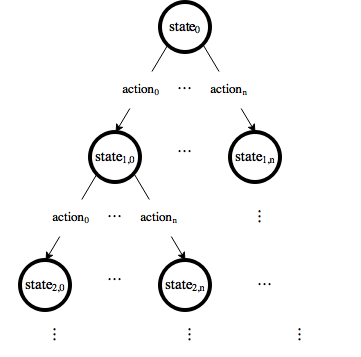
\includegraphics[scale=0.5]{include/decision_tree.png}
    \caption{A decision tree for solving a task.}
    \label{fig:dec_tree}
\end{figure}

In a typical reinforcement learning setting a problem is solved
by moving through the decision tree until a terminal state is reached.
The total result or reward of taking this exact path is then
taken into account the next time the algorithm tries to solve the problem.
The advantage of asynchronous learning is that multiple different paths
can be explored simultanously, which means that learning can happen at
a higher pace.

\subsection{Inspiration}

In december 2013 the DeepMind Technologies team published an article
about an approach to learning from a high dimensional sensory input
using deep reinforcement learning\cite{dqn}.
With a combination of convolutional nerual networks (CNN) and
the reinforcement learning method Q-learning\cite{RLbook}, they
presented results proving that it was possible to learn to play Atari
2600 games at a superhuman level.

Previously reinforcement learning haven't been able to learn to play
advanced games, but the combination of deep neural networks and
reinforcement learning have made it possible.

A problem that presents itself when a program learns to play advanced 
games is the amount of time it takes to practice.
This process is called training the algorithm and is costly in respects
to both time and computer resources.

As a way to lower the time of training the traditional reinforcement
learning algorithm can be implemented to do asynchronous training.
This way the algorithm can take advantage of modern GPUs since
they are able to execute instructions in parallel\cite{gpu_stuff}.
Learning asynchronously in this way seems straight forward in deep
reinforcement learning, since deep neural networks can be optimised
for GPU usage.

Another way to make the training asynchronous is to run multiple instances
of threads on a single CPU cluster and since almost all modern CPUs
consists of multiple cores, it is possible to have each thread run on
its own core.

An example of asynchronous reinforcement learning was presented by the
Google DeepMind team collaborating with the Montreal Institue for Learning
Algorithms (MILA) in an article from june 2016, where multiple different
reinforcement learning algorithms were implemented to take advantage of
asynchronous learning\cite{a3c}.

One of the algorithms that were implemented asynchronously
was \textit{advantage actor-critic (A3C)}, which we will use in this
project to play Atari 2600 games.

\subsection{Methods}

With the results of the A3C algorithm in mind, from the article by the
Google deepmind team\cite{a3c}, the scope of the project we present in
this paper will be to implement the actor-critic algortihm\cite{RLbook}
with a deep learning approach and extend it to exploit the benefits
of asynchronous learning.
%%%% Dette skal kun med hvis vi ikke kan gøre vores eget trådet
However, due to the time limitations of the project, we will focus on
the implementation of the actor-critic algorithm and only alter
an already existing implementation of the a3c method.
%%%%

In their first succesful attempt at learning to play Atari games using
reinforcement learning the Google deepmind team ran into problems with
the stability of their DQN-algorithm\cite{dqn} - small changes to the
weights of their network led to a large change in distribution of
visited states.
Their next article on the subject of Atari games, Asynchronous Methods for
Deep Reinforcement Learning\cite{a3c}, adressed the stability problem
and tried to solve it using an asynchronous approach.

In order to test the performance and stability of the actor-critic
method, we will be using learning environments provided by OpenAI
gym\cite{openAI} - an open source project which aims at providing
a simple interface to a collection of reinforcement learning tasks.
This collection contains a lot of Atari 2600 environments, which we will
use to compare our results to those presented in \cite{a3c}.

The main focus of this project is the stability of reinforcement learning
tasks and how asynchronous learning can be used to achieve better
stabiliyty.
We will be presenting the results of the actor-critic method used on a
simpler task than the Atari environments - the cartpole problem
\cite{cart_pole} - and then compare an asynchronous approach to the
results of the DQN-method\cite{dqn} as well as the a3c
algorithm\cite{a3c}.

In the remainder of the paper we present and review the reinforcement
learning environments in the Open AI gym collection and examine the
theory behind the reinforcement learning methods that will be used -
i.e. the actor-critic algorithm.
Furthermore, results of the actor-critic approach to solving the cart-pole
problem as well as the comparison between our asynchronous approach and
the one produced by the Google Deepmind team are given.
Lastly a discussion of these results and the stability problem as a whole
is presented as well as ideas for further work.


%\printbibliography
%\bibliography{citations}
%\bibliographystyle{plain}
\end{document}
